\documentclass[]{article}
\usepackage{lmodern}
\usepackage{amssymb,amsmath}
\usepackage{ifxetex,ifluatex}
\usepackage{fixltx2e} % provides \textsubscript
\ifnum 0\ifxetex 1\fi\ifluatex 1\fi=0 % if pdftex
  \usepackage[T1]{fontenc}
  \usepackage[utf8]{inputenc}
\else % if luatex or xelatex
  \ifxetex
    \usepackage{mathspec}
  \else
    \usepackage{fontspec}
  \fi
  \defaultfontfeatures{Ligatures=TeX,Scale=MatchLowercase}
\fi
% use upquote if available, for straight quotes in verbatim environments
\IfFileExists{upquote.sty}{\usepackage{upquote}}{}
% use microtype if available
\IfFileExists{microtype.sty}{%
\usepackage[]{microtype}
\UseMicrotypeSet[protrusion]{basicmath} % disable protrusion for tt fonts
}{}
\PassOptionsToPackage{hyphens}{url} % url is loaded by hyperref
\usepackage[unicode=true]{hyperref}
\hypersetup{
            pdftitle={gpm\_processing by Faith Musili},
            pdfborder={0 0 0},
            breaklinks=true}
\urlstyle{same}  % don't use monospace font for urls
\usepackage[margin=1in]{geometry}
\usepackage{color}
\usepackage{fancyvrb}
\newcommand{\VerbBar}{|}
\newcommand{\VERB}{\Verb[commandchars=\\\{\}]}
\DefineVerbatimEnvironment{Highlighting}{Verbatim}{commandchars=\\\{\}}
% Add ',fontsize=\small' for more characters per line
\usepackage{framed}
\definecolor{shadecolor}{RGB}{248,248,248}
\newenvironment{Shaded}{\begin{snugshade}}{\end{snugshade}}
\newcommand{\KeywordTok}[1]{\textcolor[rgb]{0.13,0.29,0.53}{\textbf{#1}}}
\newcommand{\DataTypeTok}[1]{\textcolor[rgb]{0.13,0.29,0.53}{#1}}
\newcommand{\DecValTok}[1]{\textcolor[rgb]{0.00,0.00,0.81}{#1}}
\newcommand{\BaseNTok}[1]{\textcolor[rgb]{0.00,0.00,0.81}{#1}}
\newcommand{\FloatTok}[1]{\textcolor[rgb]{0.00,0.00,0.81}{#1}}
\newcommand{\ConstantTok}[1]{\textcolor[rgb]{0.00,0.00,0.00}{#1}}
\newcommand{\CharTok}[1]{\textcolor[rgb]{0.31,0.60,0.02}{#1}}
\newcommand{\SpecialCharTok}[1]{\textcolor[rgb]{0.00,0.00,0.00}{#1}}
\newcommand{\StringTok}[1]{\textcolor[rgb]{0.31,0.60,0.02}{#1}}
\newcommand{\VerbatimStringTok}[1]{\textcolor[rgb]{0.31,0.60,0.02}{#1}}
\newcommand{\SpecialStringTok}[1]{\textcolor[rgb]{0.31,0.60,0.02}{#1}}
\newcommand{\ImportTok}[1]{#1}
\newcommand{\CommentTok}[1]{\textcolor[rgb]{0.56,0.35,0.01}{\textit{#1}}}
\newcommand{\DocumentationTok}[1]{\textcolor[rgb]{0.56,0.35,0.01}{\textbf{\textit{#1}}}}
\newcommand{\AnnotationTok}[1]{\textcolor[rgb]{0.56,0.35,0.01}{\textbf{\textit{#1}}}}
\newcommand{\CommentVarTok}[1]{\textcolor[rgb]{0.56,0.35,0.01}{\textbf{\textit{#1}}}}
\newcommand{\OtherTok}[1]{\textcolor[rgb]{0.56,0.35,0.01}{#1}}
\newcommand{\FunctionTok}[1]{\textcolor[rgb]{0.00,0.00,0.00}{#1}}
\newcommand{\VariableTok}[1]{\textcolor[rgb]{0.00,0.00,0.00}{#1}}
\newcommand{\ControlFlowTok}[1]{\textcolor[rgb]{0.13,0.29,0.53}{\textbf{#1}}}
\newcommand{\OperatorTok}[1]{\textcolor[rgb]{0.81,0.36,0.00}{\textbf{#1}}}
\newcommand{\BuiltInTok}[1]{#1}
\newcommand{\ExtensionTok}[1]{#1}
\newcommand{\PreprocessorTok}[1]{\textcolor[rgb]{0.56,0.35,0.01}{\textit{#1}}}
\newcommand{\AttributeTok}[1]{\textcolor[rgb]{0.77,0.63,0.00}{#1}}
\newcommand{\RegionMarkerTok}[1]{#1}
\newcommand{\InformationTok}[1]{\textcolor[rgb]{0.56,0.35,0.01}{\textbf{\textit{#1}}}}
\newcommand{\WarningTok}[1]{\textcolor[rgb]{0.56,0.35,0.01}{\textbf{\textit{#1}}}}
\newcommand{\AlertTok}[1]{\textcolor[rgb]{0.94,0.16,0.16}{#1}}
\newcommand{\ErrorTok}[1]{\textcolor[rgb]{0.64,0.00,0.00}{\textbf{#1}}}
\newcommand{\NormalTok}[1]{#1}
\usepackage{graphicx,grffile}
\makeatletter
\def\maxwidth{\ifdim\Gin@nat@width>\linewidth\linewidth\else\Gin@nat@width\fi}
\def\maxheight{\ifdim\Gin@nat@height>\textheight\textheight\else\Gin@nat@height\fi}
\makeatother
% Scale images if necessary, so that they will not overflow the page
% margins by default, and it is still possible to overwrite the defaults
% using explicit options in \includegraphics[width, height, ...]{}
\setkeys{Gin}{width=\maxwidth,height=\maxheight,keepaspectratio}
\IfFileExists{parskip.sty}{%
\usepackage{parskip}
}{% else
\setlength{\parindent}{0pt}
\setlength{\parskip}{6pt plus 2pt minus 1pt}
}
\setlength{\emergencystretch}{3em}  % prevent overfull lines
\providecommand{\tightlist}{%
  \setlength{\itemsep}{0pt}\setlength{\parskip}{0pt}}
\setcounter{secnumdepth}{0}
% Redefines (sub)paragraphs to behave more like sections
\ifx\paragraph\undefined\else
\let\oldparagraph\paragraph
\renewcommand{\paragraph}[1]{\oldparagraph{#1}\mbox{}}
\fi
\ifx\subparagraph\undefined\else
\let\oldsubparagraph\subparagraph
\renewcommand{\subparagraph}[1]{\oldsubparagraph{#1}\mbox{}}
\fi

% set default figure placement to htbp
\makeatletter
\def\fps@figure{htbp}
\makeatother


\title{gpm\_processing by Faith Musili}
\author{}
\date{\vspace{-2.5em}}

\begin{document}
\maketitle

\subsection{Introduction}\label{introduction}

The official
\href{https://pmm.nasa.gov/sites/default/files/document_files/IMERG_doc_190909.pdf}{technical
report} describes in details all aspects of GPM IMERG product.

It's worth noting that these images are both trmm and gpm layers
together with an overlap. Trmm images have 25km resolution while Gpm
have a 10km resolution.

\begin{Shaded}
\begin{Highlighting}[]
\KeywordTok{library}\NormalTok{(raster)}
\KeywordTok{library}\NormalTok{(gdalUtils)}
\KeywordTok{library}\NormalTok{(tidyr)}
\end{Highlighting}
\end{Shaded}

\subsection{1. Data download}\label{data-download}

GPM data download hit several barriers because they prohibited online
ftp download . This meant functions in R like rcurl\_download() nolonger
works.

Therefore, to download this data.

\begin{enumerate}
\def\labelenumi{\arabic{enumi}.}
\item
  Log into \href{https://urs.earthdata.nasa.gov/}{Earthdata}
\item
  After sucessful log in, go to
  \href{https://search.earthdata.nasa.gov/search}{Earthdata search} and
  search for \textbf{IMERG}
\end{enumerate}

3.Select monthly product
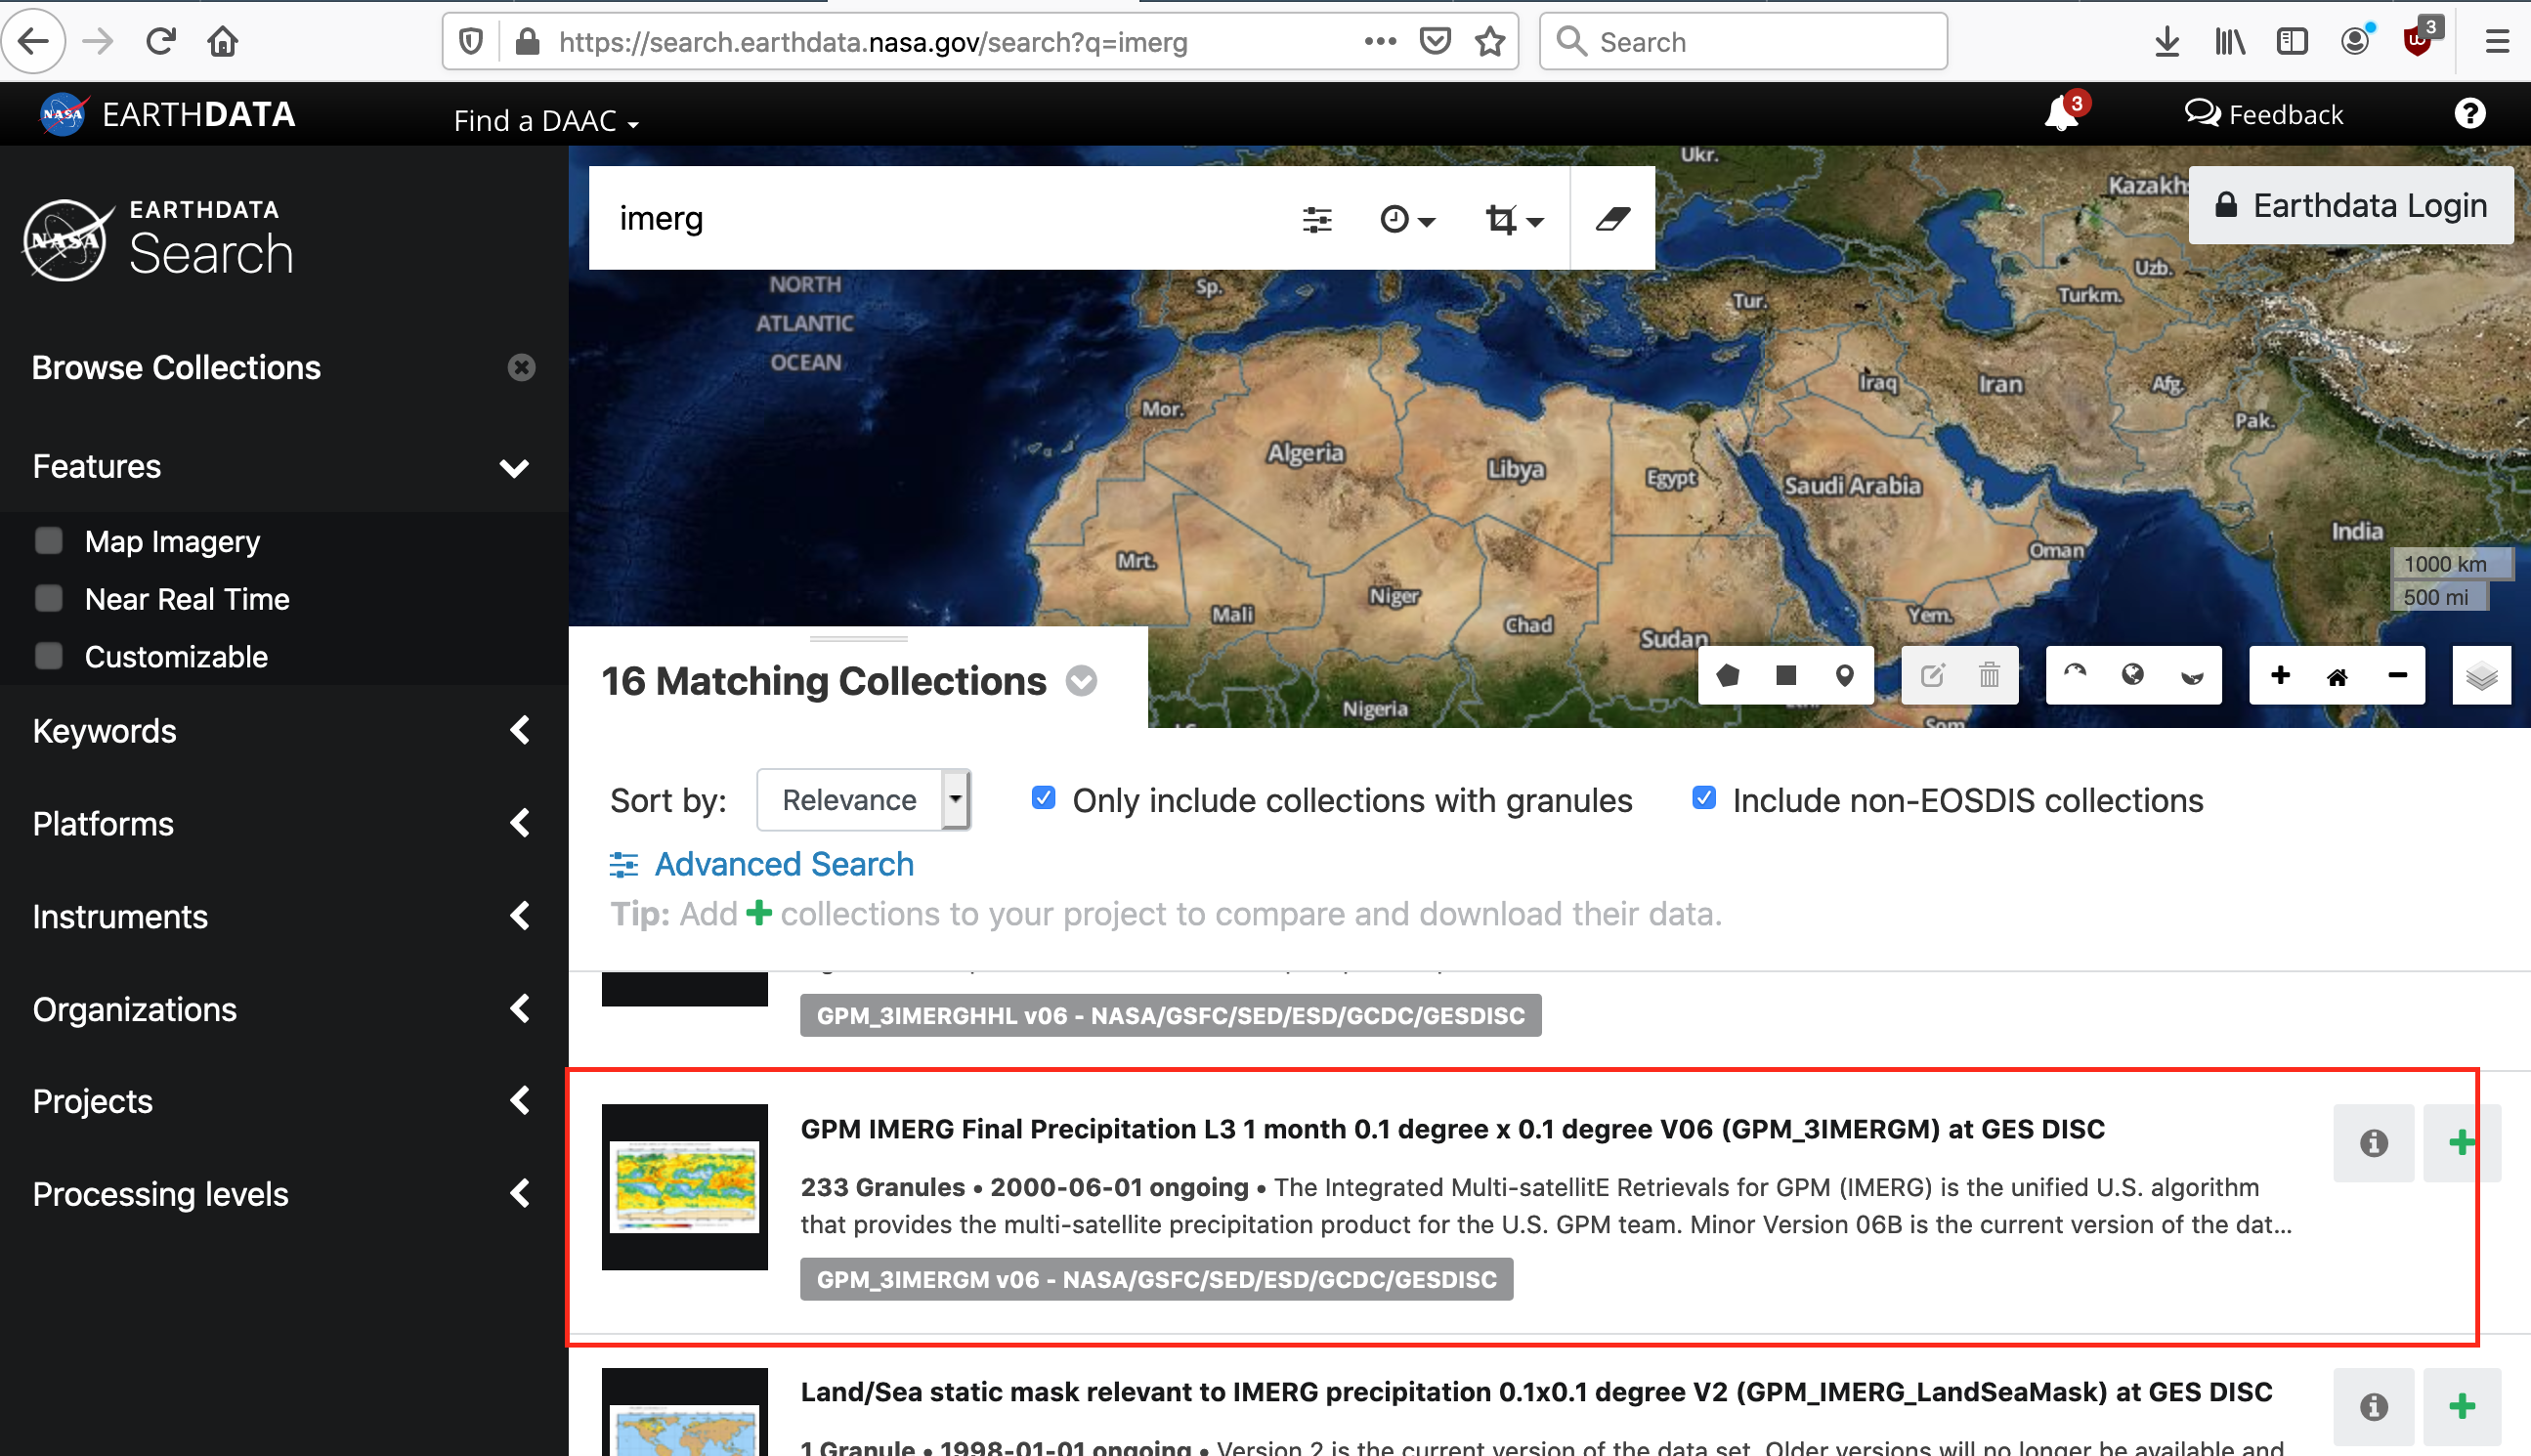
\includegraphics{/media/pogo2/data/GPM_faith/select_product.png}

4.Then press ``Download all button''(if you wish to download all the
data, if not, choose what you want.)

\begin{enumerate}
\def\labelenumi{\arabic{enumi}.}
\setcounter{enumi}{4}
\tightlist
\item
  After page redirects, choose ``Direct Download'' then ``Done'' then
  ``Download data''.
\end{enumerate}

6.On the new page, select ``View/Download data links''
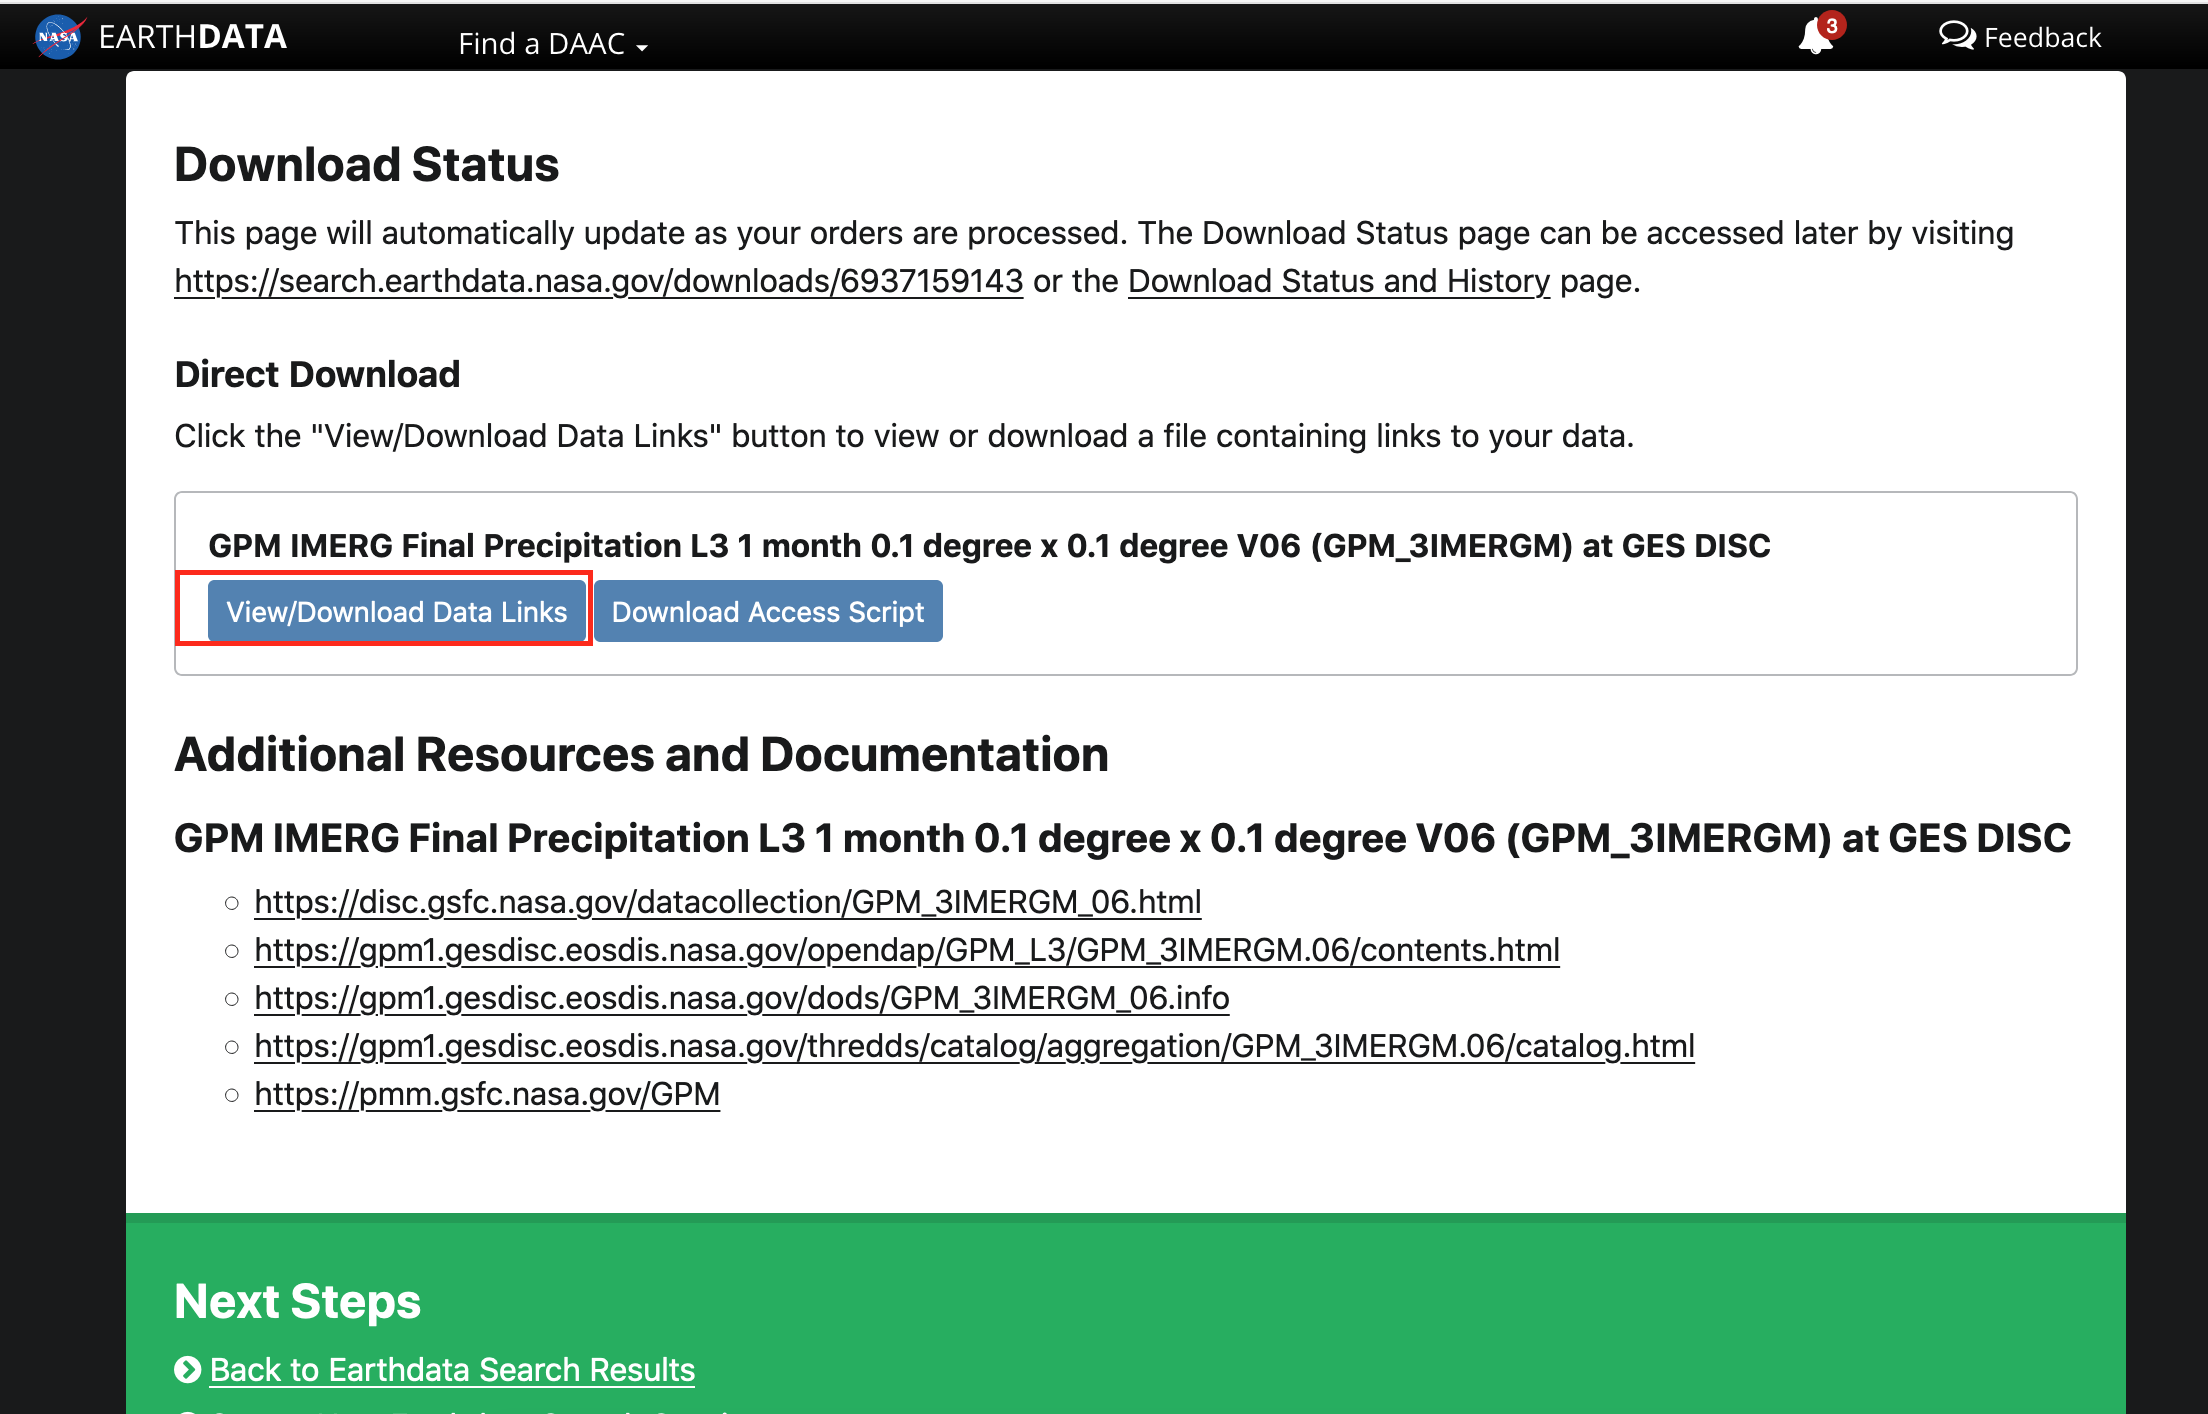
\includegraphics{/media/pogo2/data/GPM_faith/links.png}

7.Select ``Download Links File'' and save your text filee.g
``mylinks.txt''

\begin{enumerate}
\def\labelenumi{\arabic{enumi}.}
\setcounter{enumi}{7}
\item
  On you local machine/server terminal, go to the location you want to
  write the GPM images.
\item
  Run the following command \textbf{``wget --content-disposition
  --load-cookies \textasciitilde{}/.urs\_cookies --save-cookies
  \textasciitilde{}/.urs\_cookies --keep-session-cookies
  --content-disposition -i {[}mylinks.txt{]}''}
\end{enumerate}

\subsection{2. Conversion of HDF files to
tif}\label{conversion-of-hdf-files-to-tif}

From gdalinfo()
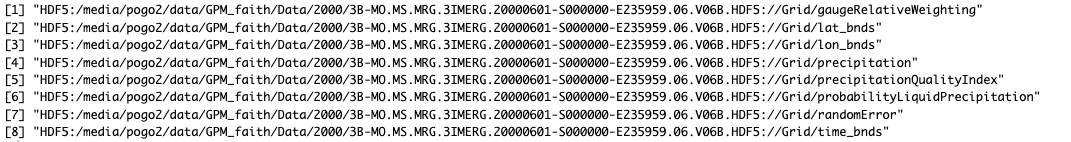
\includegraphics{/media/pogo2/data/GPM_faith/gpm_subdatasets.png} and to
get precipitation amounts we used subdataset 4
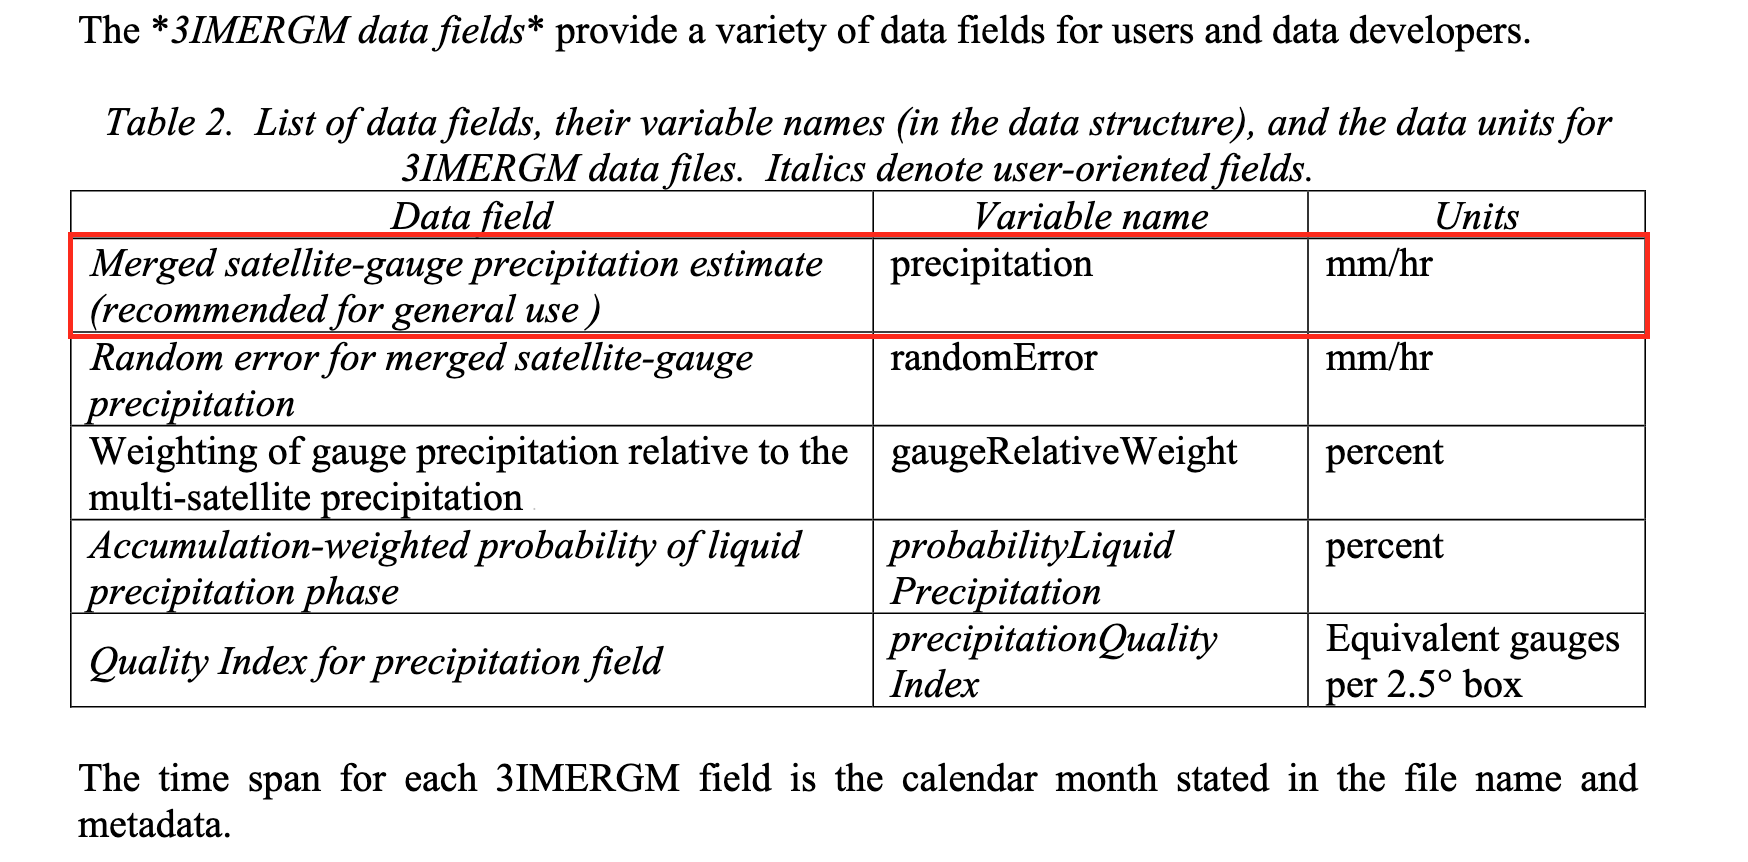
\includegraphics{/media/pogo2/data/GPM_faith/GPM_subset_details.png}

\begin{Shaded}
\begin{Highlighting}[]
\KeywordTok{setwd}\NormalTok{(}\StringTok{"/media/pogo2/data/GPM_faith"}\NormalTok{)## set the working directory ( where the HDF files are)}

\NormalTok{files <-}\StringTok{ }\KeywordTok{list.files}\NormalTok{(}\DataTypeTok{pattern=}\StringTok{"*.HDF"}\NormalTok{,}\DataTypeTok{full.names =} \OtherTok{FALSE}\NormalTok{,}\DataTypeTok{recursive =} \OtherTok{TRUE}\NormalTok{)## list all HDF files in that directory}

\NormalTok{## convert .HDF files to .tif (i.e the 4th subdataset which is precipitation as per documentation)}
\ControlFlowTok{for}\NormalTok{ (filename }\ControlFlowTok{in}\NormalTok{ files)\{}
\NormalTok{  sds <-}\StringTok{ }\KeywordTok{get_subdatasets}\NormalTok{(filename)}
  \KeywordTok{gdal_translate}\NormalTok{(sds[}\DecValTok{4}\NormalTok{], }\DataTypeTok{dst_dataset=}\KeywordTok{paste0}\NormalTok{(}\KeywordTok{substr}\NormalTok{(filename, }\DecValTok{1}\NormalTok{, }\KeywordTok{nchar}\NormalTok{(filename)}\OperatorTok{-}\DecValTok{5}\NormalTok{) ,}\StringTok{".tif"}\NormalTok{))}
\NormalTok{\}}
\end{Highlighting}
\end{Shaded}

\subsection{3. Create a raster brick from all the monthly
layers}\label{create-a-raster-brick-from-all-the-monthly-layers}

\begin{Shaded}
\begin{Highlighting}[]
\NormalTok{## stack all months together}
\KeywordTok{setwd}\NormalTok{(}\StringTok{"/media/pogo2/data/GPM_faith"}\NormalTok{)}
\NormalTok{gpm<-}\KeywordTok{list.files}\NormalTok{(}\DataTypeTok{pattern =}\StringTok{"*.tif"}\NormalTok{ ,}\DataTypeTok{recursive =} \OtherTok{TRUE}\NormalTok{,}\DataTypeTok{full.names =} \OtherTok{TRUE}\NormalTok{)}
\NormalTok{gpmBrick<-}\KeywordTok{brick}\NormalTok{(}\KeywordTok{lapply}\NormalTok{(gpm,raster))}
\KeywordTok{names}\NormalTok{(gpmBrick)<-}\KeywordTok{paste0}\NormalTok{(}\StringTok{"gpm_"}\NormalTok{,}\DecValTok{1}\OperatorTok{:}\KeywordTok{nlayers}\NormalTok{(gpmBrick))}

\KeywordTok{writeRaster}\NormalTok{(gpmBrick,}\StringTok{"gpmbrick.tif"}\NormalTok{,}\DataTypeTok{format=}\StringTok{"GTiff"}\NormalTok{, }\DataTypeTok{overwrite=}\OtherTok{TRUE}\NormalTok{)}
\end{Highlighting}
\end{Shaded}

\subsection{4. Georefrence the raster stack(in
QGIS)}\label{georefrence-the-raster-stackin-qgis}

This GPM stack is not georefrenced and i didn't find a way to do it in R
so i used QGIS to reorefrence it. From the gdalinfo() document,
following are the bounding coordinates to be used in georefrencing: -
NorthBoundingCoordinate=90 - SouthBoundingCoordinate=-90 -
EastBoundingCoordinate=180 - WestBoundingCoordinate=-180

\subsection{5. Convert all -9999 or -9999.9 (missing data) to
0}\label{convert-all--9999-or--9999.9-missing-data-to-0}

As per the
\href{https://pmm.nasa.gov/sites/default/files/document_files/IMERG_doc_190909.pdf}{documentation}
on page 64:

\textbf{``All products in IMERG use the \emph{standard missing
value}''-9999.9``or ???-9999??? for 4-byte floats or 2-byte integers,
respectively.Thesevalues are carried in the metadata.''}

\begin{Shaded}
\begin{Highlighting}[]
\NormalTok{brick<-}\KeywordTok{brick}\NormalTok{(}\StringTok{"/Users/FMusili/Desktop/gpmbrick_modified.tif"}\NormalTok{)## read in georefrenced brick ( the georefrencing was done in QGIS)}
\NormalTok{brick.new<-}\StringTok{ }\KeywordTok{calc}\NormalTok{(brick, }\DataTypeTok{fun=}\ControlFlowTok{function}\NormalTok{(x) \{ x[x}\OperatorTok{<}\DecValTok{0}\NormalTok{] <-}\StringTok{ }\DecValTok{0}\NormalTok{; }\KeywordTok{return}\NormalTok{(x)\})## replace all values less than zero with zero }
\end{Highlighting}
\end{Shaded}

\subsection{6. Convert the precipitation to mm from mm/hr for all
monthly
layers}\label{convert-the-precipitation-to-mm-from-mmhr-for-all-monthly-layers}

According to
\href{https://pmm.nasa.gov/sites/default/files/document_files/IMERG_doc_190909.pdf}{documentation}
the precipitation layer is in mm/hr.
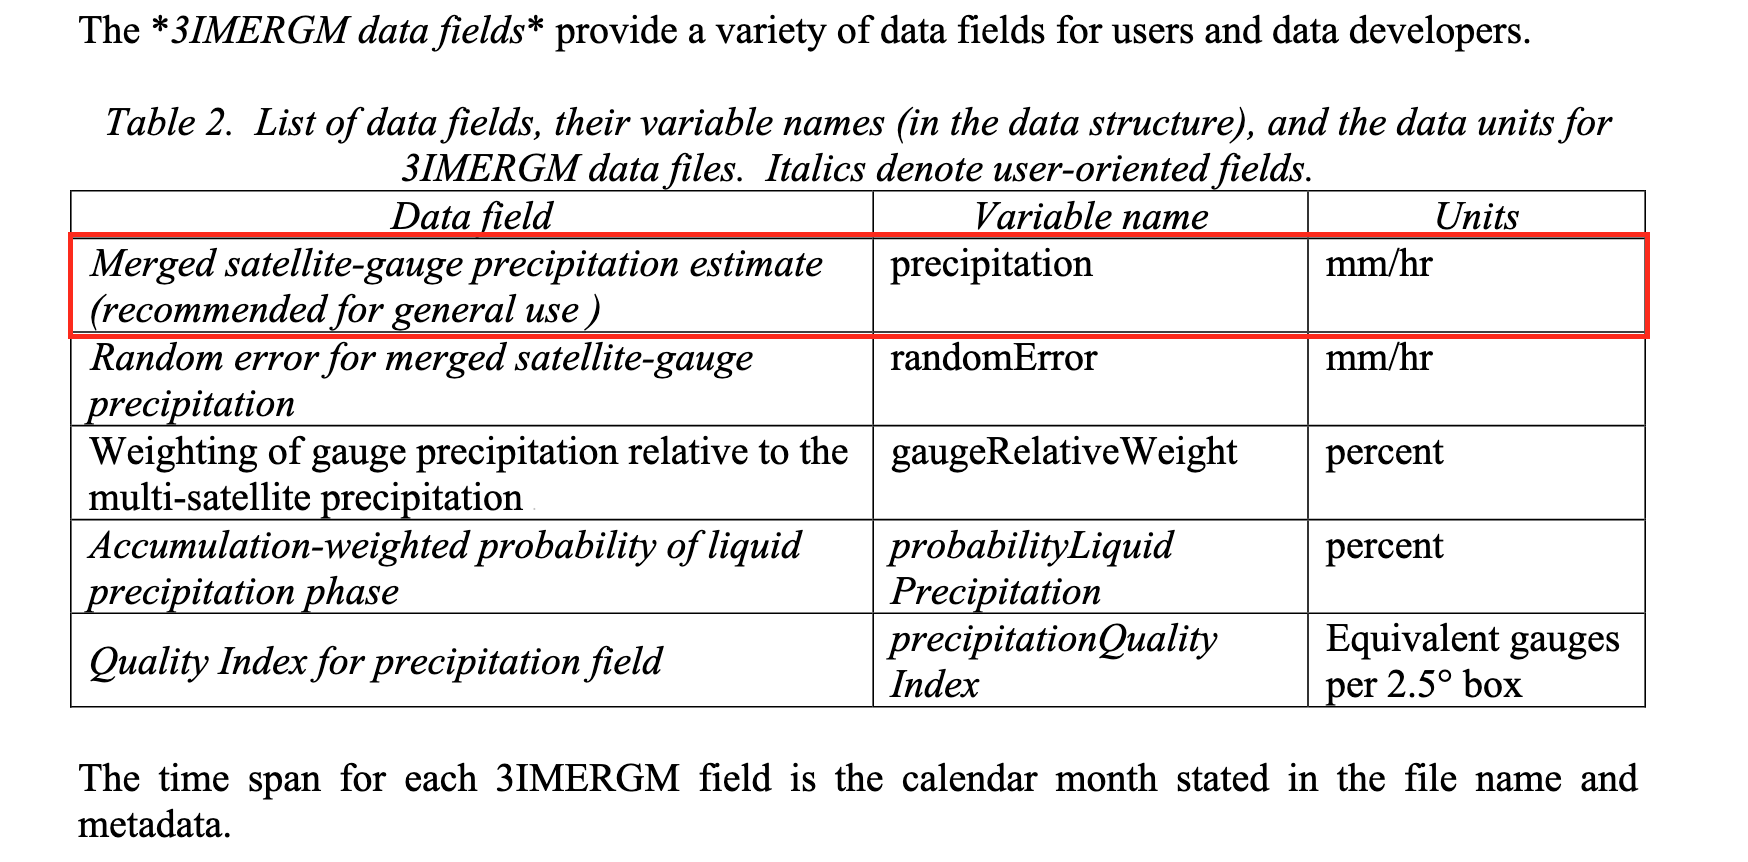
\includegraphics{/media/pogo2/data/GPM_faith/GPM_subset_details.png}

This being a monthly product to convert mm/hr to mm, we muliply number
of days in that month*24hrs.

\textbf{It should be noted that this product has data from June 2000 to
October 2019}

\begin{Shaded}
\begin{Highlighting}[]
\NormalTok{## function to retrive number of days in each month}
\NormalTok{numDays <-}\StringTok{ }\ControlFlowTok{function}\NormalTok{(month,year)\{}
  \KeywordTok{as.numeric}\NormalTok{(}\KeywordTok{strftime}\NormalTok{(}\KeywordTok{as.Date}\NormalTok{(}\KeywordTok{paste}\NormalTok{(year}\OperatorTok{+}\NormalTok{month}\OperatorTok\DecValTok{12}\NormalTok{,month}\OperatorTok\DecValTok{12}\OperatorTok{+}\DecValTok{1}\NormalTok{,}\StringTok{"01"}\NormalTok{,}\DataTypeTok{sep=}\StringTok{"-"}\NormalTok{))}\OperatorTok{-}\DecValTok{1}\NormalTok{,}\StringTok{"%d"}\NormalTok{))}
\NormalTok{\}}

\NormalTok{monthdays<-}\KeywordTok{sapply}\NormalTok{(}\DecValTok{1}\OperatorTok{:}\DecValTok{12}\NormalTok{,numDays,}\DecValTok{2000}\OperatorTok{:}\DecValTok{2019}\NormalTok{)}\OperatorTok\NormalTok{## list all month days from 2000 to 2019}
\StringTok{  }\KeywordTok{data.frame}\NormalTok{()}\OperatorTok
\StringTok{  }\KeywordTok{mutate}\NormalTok{(}\DataTypeTok{Year=}\DecValTok{2000}\OperatorTok{:}\DecValTok{2019}\NormalTok{)## add year column}
\KeywordTok{names}\NormalTok{(monthdays)[}\DecValTok{1}\OperatorTok{:}\DecValTok{12}\NormalTok{]<-month.name## rename columns}


\NormalTok{monthdays<-monthdays}\OperatorTok\KeywordTok{pivot_longer}\NormalTok{(January}\OperatorTok{:}\NormalTok{December,}\DataTypeTok{names_to =} \StringTok{"month"}\NormalTok{,}\DataTypeTok{values_to =} \StringTok{"days"}\NormalTok{)## reshape}
\NormalTok{monthdays<-monthdays[}\OperatorTok{-}\KeywordTok{c}\NormalTok{(}\DecValTok{1}\OperatorTok{:}\DecValTok{5}\NormalTok{,}\DecValTok{239}\OperatorTok{:}\DecValTok{240}\NormalTok{),]## remove missing layers months}
\NormalTok{monthdays.time<-monthdays}\OperatorTok\KeywordTok{mutate}\NormalTok{(}\DataTypeTok{hours=}\NormalTok{days}\OperatorTok{*}\DecValTok{24}\NormalTok{)## multiply each number of days by 24 hours.}

\NormalTok{##  multiply each monthly layer by corresponding days*24hrs because the rainfall is in mm/hr as per the GPM documentation}
\ControlFlowTok{for}\NormalTok{(i }\ControlFlowTok{in} \DecValTok{1}\OperatorTok{:}\KeywordTok{nrow}\NormalTok{(monthdays.time)) \{}
\NormalTok{  brick.new[[i]]  <-}\StringTok{ }\NormalTok{brick.new[[i]] }\OperatorTok{*}\StringTok{ }\NormalTok{monthdays.time}\OperatorTok{$}\NormalTok{hours[i]}
\NormalTok{\}}

\KeywordTok{writeRaster}\NormalTok{(brick.new,}\StringTok{"/Users/FMusili/Desktop/gpmbrick_final.tif"}\NormalTok{,}\DataTypeTok{format=}\StringTok{"GTiff"}\NormalTok{)## write out the final global monthly stack}
\end{Highlighting}
\end{Shaded}

\end{document}
